\chapter{\xlabel{pol2_overview}POL-2 Overview}
\label{sec:pol2}
\section{\xlabel{pol2}The instrument}

The POL-2 instrument is a linear polarimetry module for the
Submillimetre Common User Bolometer Array-2 (SCUBA-2), a 10,000
bolometer camera on the JCMT \cite{Friberg} \cite{Bastien2011}.  POL-2
in itself is not a detector - thus requiring SCUBA-2 and its detectors
for operation. SCUBA-2 operates simultaneously at both 850 and
\SI{450}{\micro\metre}. The POL-2 instrument is currently commissioned
at \SI{850}{\micro\metre} only.

\begin{figure}[t!]
\begin{center}
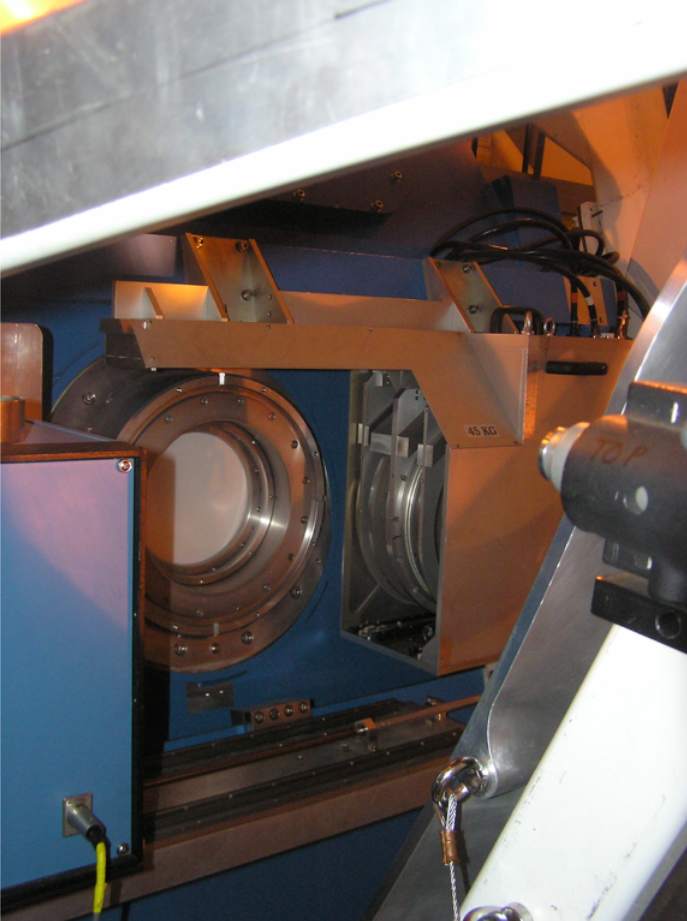
\includegraphics[width=0.45\linewidth]{pol2-out-of-beam.png}
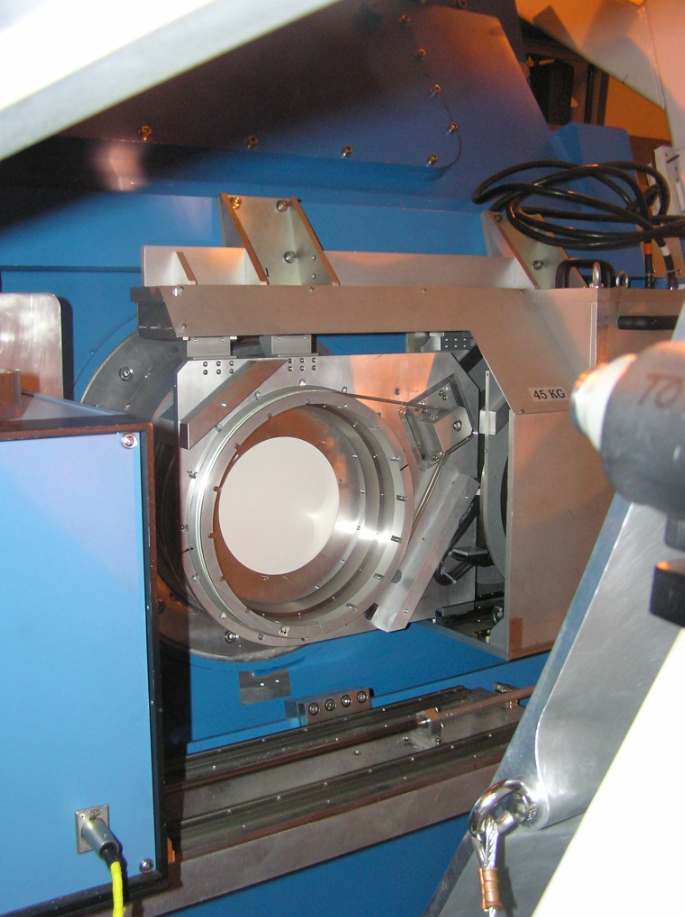
\includegraphics[width=0.45\linewidth]{pol2-in-beam.png}
\label{fig:pol2sc2}
\caption [POL-2 mounted on SCUBA-2]{POL-2 mounted on the front of
  SCUBA-2.  The left image shows the SCUBA-2 window. The right image
  shows the components of POL-2 inserted in front of the SCUBA-2
  window: the calibrator grid, rotating half-wave-plate (HWP) and the
  analyser grid. The calibrator grid is only inserted for test
  purposes.}
\end{center}
\end{figure}

\subsection*{Polarisation}

In polarimetric terms light is conventionally described by the four
Stokes parameters: $I$, $Q$, $U$ and $V$.


$I$ is the total intensity; $Q$ is the radiation linearly polarised in
the direction parallel or perpendicular to the reference plane. $U$ is
the radiation linearly polarised in the directions 45$^{\circ }$ to
the reference plane; and $V$ is the circularly polarised radiation.

POL-2 is designed to characterize linear polarisation.  The $V$
parameter, consequently, is not discussed further with the focus on $I$,
$Q$ and $U$.

The linear Polarised Intensity (I$_{p}$) and  polarisation angle
($\theta$) can be described as:

\begin{equation}
I_{p} = \sqrt{Q^{2}+U^{2}}
\end{equation}
\begin{equation}
\theta = 0.5\arctan(U/Q)
\end{equation}

with Q and U related to the polarisation angle and the polarised intensity by:

\begin{equation}
Q = I_{p} \text{cos}(2\theta)
\end{equation}
\begin{equation}
U = I_{p} \text{sin}(2\theta)
\end{equation}

where

\begin{equation}
Q = Q_{m} - I . IP_{q}
\end{equation}
\begin{equation}
U = U_{m} - I . IP_{u}
\end{equation}

where Q$_{m}$ and U$_{m}$ are the measured values of Q and U.  I is
the astronomical total intensity.  IP is the instrumental
polarisation. The IP affects both Q (\emph{via} IP$_{q}$) and U
(\emph{via} IP$_{u}$).


\subsection*{How POL-2 works}

POL-2 is located in front of the window to the SCUBA-2 instrument (as
is seen in Figure~\ref{fig:pol2sc2}), and covers the full field of
view of SCUBA-2. The POL-2 polarimeter uses three optical components
that cover the full field of SCUBA-2:

\begin{enumerate}
\item a wire-grid polariser used as a calibrator (only included in the
  beam for test purposes)
\item a Half-Wave Plate (HWP)
\item a second wire-grid polariser used as an analyser
\end{enumerate}

These components can be seen in Figure~\ref{fig:pol2sc2}.  A schematic
of POL-2 is given in Figure~\ref{fig:pol2sc2diagram}.

\begin{figure}[t!]
\begin{center}
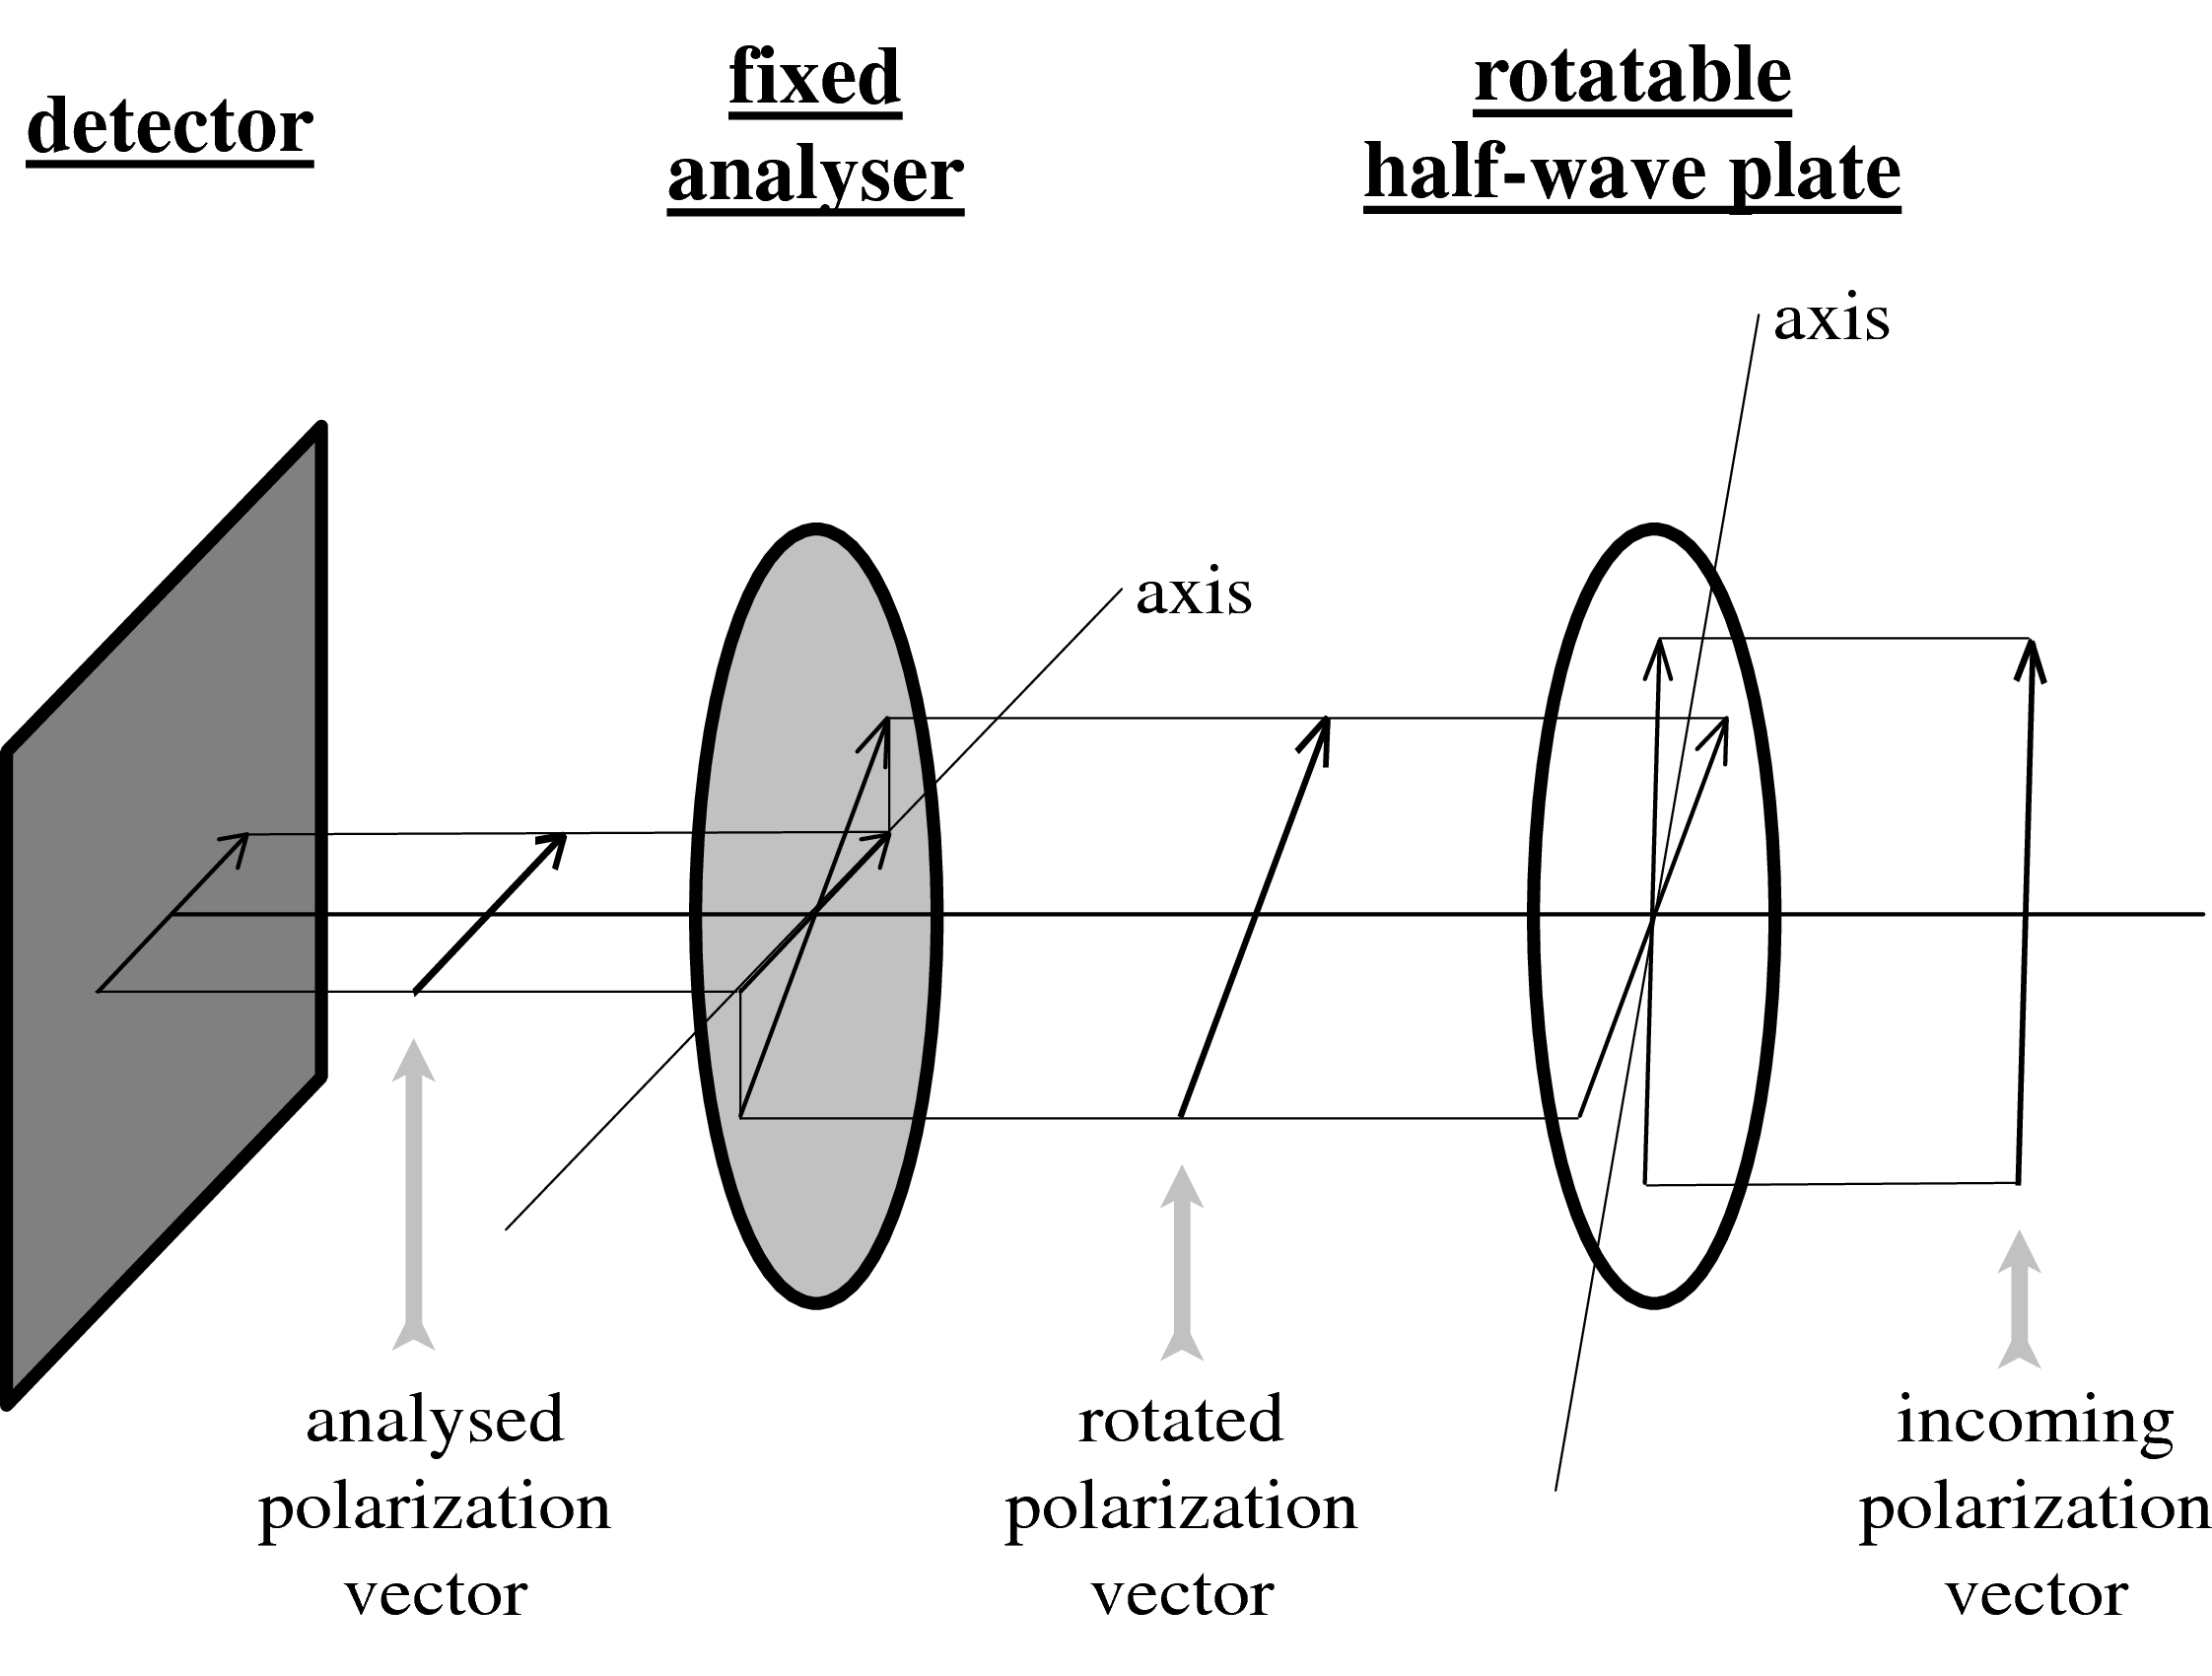
\includegraphics[width=0.8\linewidth]{singopt.png}
\caption [POL-2 optical components]{ The main optical components in a
  typical single-beam imaging polarimeter such as POL-2 (taken from
  SUN/223).}
\label{fig:pol2sc2diagram}
\end{center}
\end{figure}

Rotating the HWP rotates any linearly polarised component of incoming
radiation. The HWP rotates this incoming linear polarisation with
twice the speed of the HWP angle ($\delta$) producing the
\emph{effective analyser} position ($\phi$ - as defined in
\xref{the POLPACK documentation}{sun223} {thepolarimeter}), such that:


\begin{equation}
\phi = 2 \delta
\end{equation}


The rotating linearly polarised component is transmitted or reflected
by the grid, causing a modulation in the transmitted intensity.
The amplitude of the polarised component transmitted by the polariser is
$\sim$cos($\phi$) while the power is $\sim$cos$^{2}$($\phi$).

\begin{figure}[t!]
\begin{center}
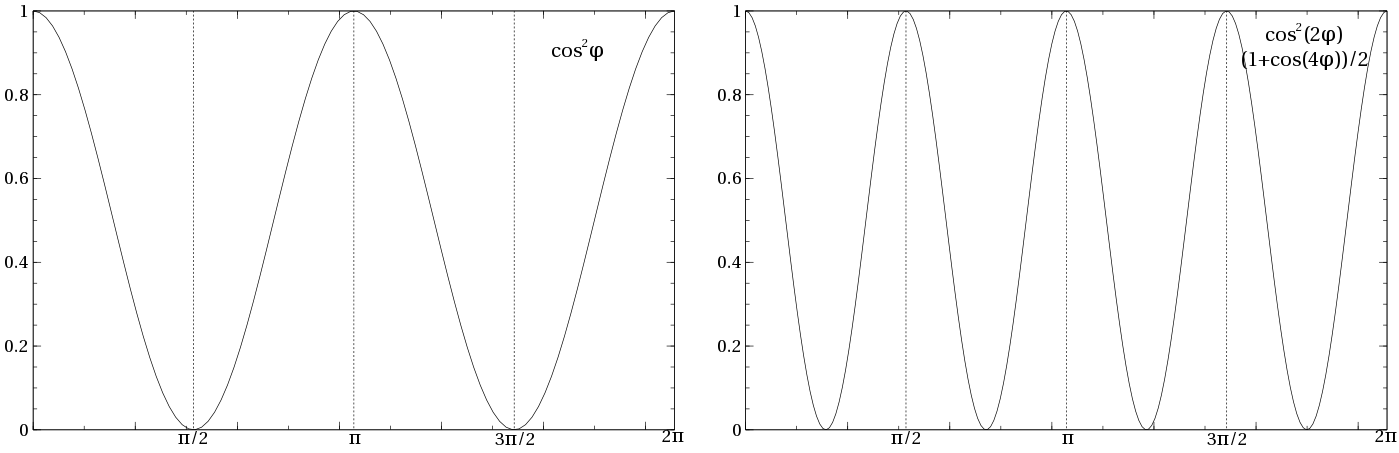
\includegraphics[width=0.95\linewidth]{hwp-modulation-basic.png}
\label{fig:hwp-modulation-basic}
\caption [Modulation by the HWP - basic description]{ Left: If there
  was a single rotating analyser this would be the resulting curve of
  the power transmitted of the linearly polarised component.
  Right: With the HWP the linearly polarised component is
  rotated at twice the speed. It may be useful to remind the reader of
  the trigonometric identity: \\ cos$^{2}$x = 0.5(1+cos(2x))}
\end{center}
\end{figure}


The radiation passing through the polarimeter is detected by
SCUBA-2. The detected intensity (I$_{detected}$) is a combination of
\emph{both} the unpolarised intensity (I$_{unpolarised}$) and the
linearly polarised intensity (I$_{p}$)\footnote{The total intensity of
the source, $I$, is $I_{unpolarised} + I_{p}$.}. This detected intensity can be
described by:

\begin{equation}
I_{detected} = \frac{I_{unpolarised}}{2}+ I_{p}\cdot\left(\frac{1+\cos(2\phi - 2\theta)}{2} \right)
\end{equation}

with the above equation being in terms of the effective analyser
angle, $\phi$ and the angle of the polarisation ($\theta)$.
This can also be expressed in terms of the  the HWP angle ($\delta$).

\begin{equation}
\label{eqn:idet}
I_{detected} = \frac{I_{unpolarised}}{2}+I_{p}\cdot\left(\frac{1+\cos(4\delta - 2\theta)}{2} \right)
\end{equation}




\subsection*{The Half-Wave Plate}

As described in the POL-2 commissioning document the HWP is
constructed from five individual synthetic sapphire layers
approximately 0.9 mm thick and 200 mm in diameter. The transmission
properties of sapphire are generally good at the SCUBA-2 wavelengths
but are dependent on the thickness and ambient temperature. The total
effective transmission of the HWP integrated across the 850 and
\SI{450}{\micro\metre} filter bands are about 86\% and 57\%
respectively (Savini et al. 2009 - insert full reference).

The HWP rotates the incoming linear polarisation with twice the speed
of the wave plate angle.  The HWP is typically rotated at 2Hz,
providing a fast modulation of any linear polarisation by 8Hz (see
equation~\ref{eqn:idet}).  The data acquisition rate is ~175Hz, yielding
20 samples per cycle.  The atmosphere is stable on the order of 2Hz and
can be removed.


\begin{figure}[t!]
\begin{center}
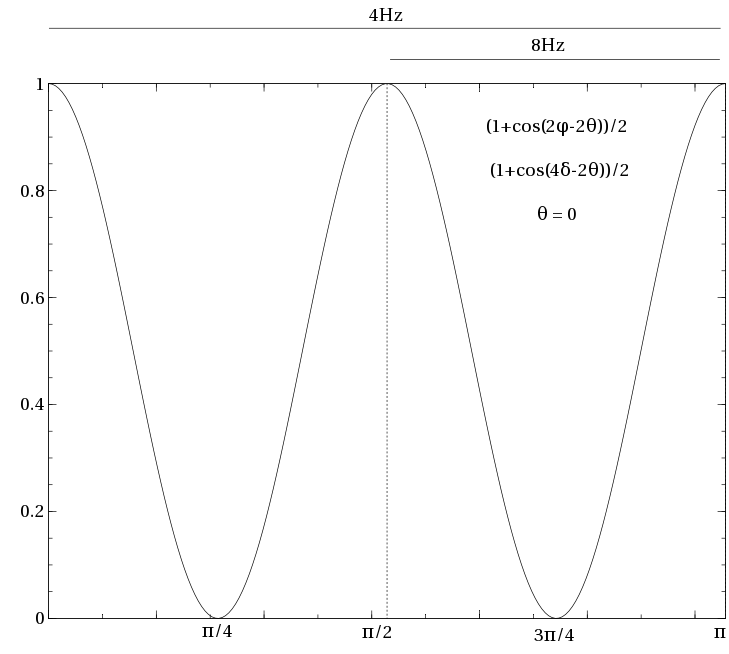
\includegraphics[width=0.7\linewidth]{hwp-modulation.png}
\label{fig:hwpmodulation}
\caption [Attenuation of signal by HWP]{The incoming polarised
  radiation (with a polarised angle, $\theta$, of zero) is attenuated
  by the HWP.  The HWP rotates at 2Hz (through $2\pi$) so we see the
  signal is modulated at 8Hz as the instrument scans at
  8\si{\arcsecond}/s. }
\end{center}
\end{figure}


\begin{figure}[t!]
\begin{center}
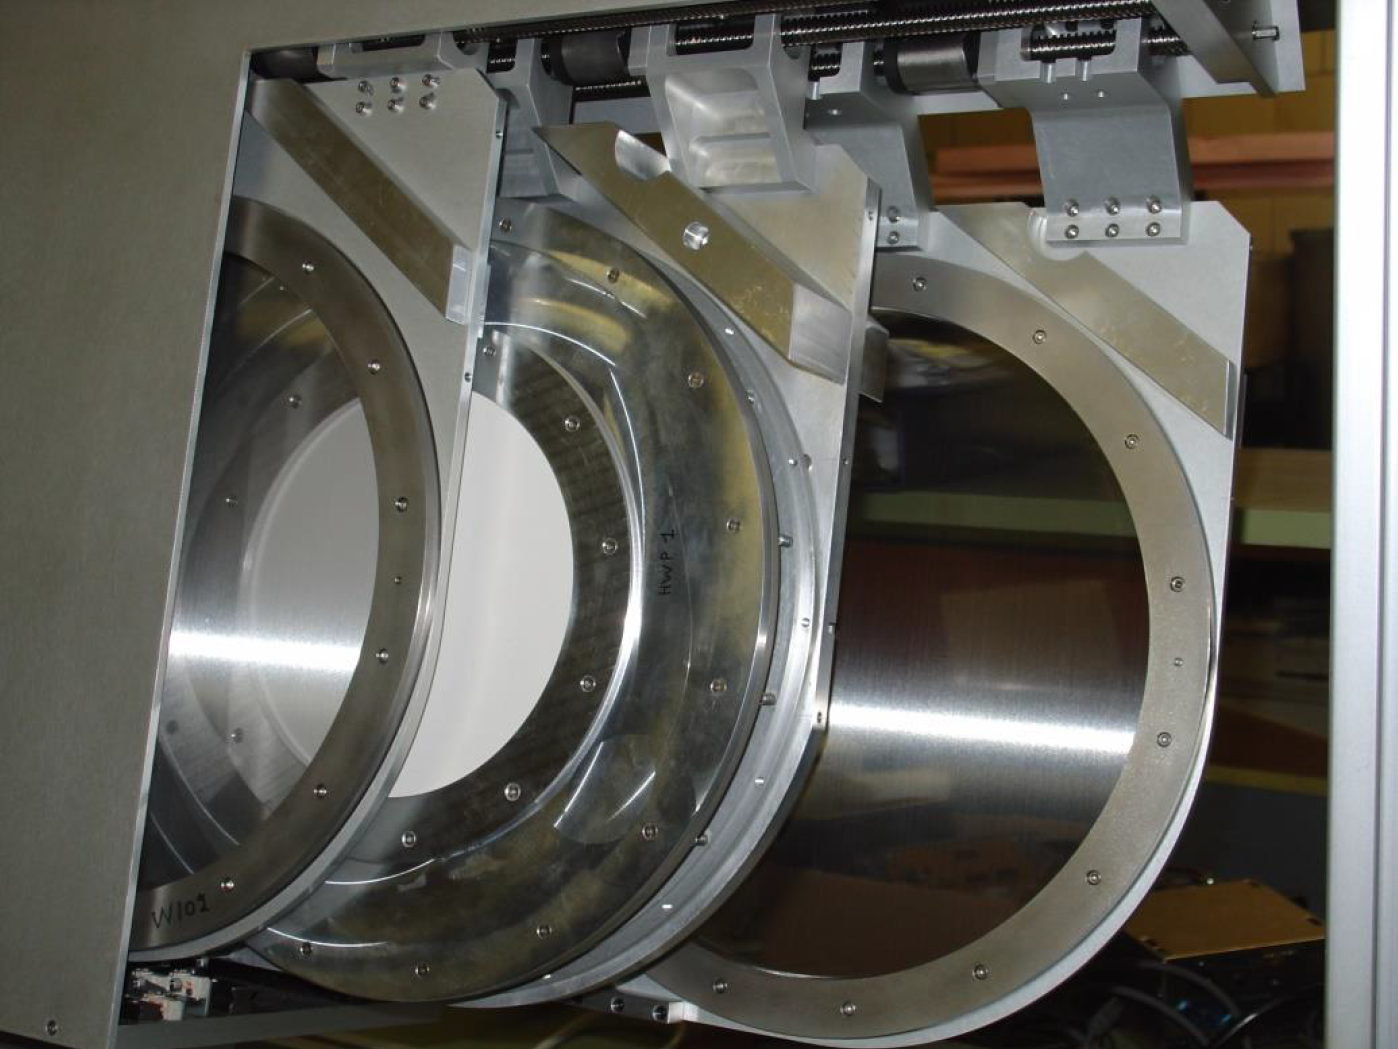
\includegraphics[width=0.7\linewidth]{pol2-three-components.png}
\label{fig:pol2components}
\caption [POL-2 components]{
  The three blades that combine to form POL-2 are partially
  extended showing the two wire grids and the achromatic HWP.
  The two wire grids are the calibrator grid and the analyser grid.
  The rotating HWP is located between these two fixed grids.
  The calibrator grid is only inserted for test purposes.
  Stiffeners can be seen on all three blades. The one for the HWP
  is particularly thick. Their purpose is to reduce vibrations while
  the HWP spins.
}
\end{center}
\end{figure}




\section{Instrumental Polarisation}
\label{sec:ip}

At the angular resolution of JCMT, planets such as Uranus should
appear as unpolarised point sources.  In practice, however, POL-2
observations of such sources exhibit a measurable level of
polarisation - albeit typically less than 1.5\% at 850 $\mu$m. This
is evidence that some part of the incoming astronomical radiation is
being partially polarised by one or more of the components of the
telescope/POL-2/SCUBA-2 that are in the light path. This polarisation
is referred to as "Instrumental Polarisation" (IP).

In order to establish the true Q and U from an astronomical source, it
is necessary to correct for this effect. For the case of a low degree
of polarisation in the incoming radiation and a low degree of IP, the
following is a good approximation for correcting the measurement for
the effects of the IP:

\begin{equation}
Q = Q_{m} - I. ip_{q}
\end{equation}

\begin{equation}
U = U_{m} - I. ip_{u}
\end{equation}

where $Q_{m}$ and $U_{m}$ are the measured values for a single
bolometer sample at some point on the sky. $Q$ and $U$ are the true
(corrected) values, $I$ is the astronomical total intensity at the same
point on the sky (i.e. the total intensity after removal of the sky
and electronic backgrounds) and $ip_{q}$ and $ip_{u}$ are factors that
may vary slowly with focal plane position and/or azimuth and
elevation.

IP correction of a POL-2 map therefore requires a total
intensity map of the same area of the sky to be available. This total
intensity map is referred to as the IP reference map.

Whilst flat mirrors or surfaces will produce a small, constant
polarisation across the beam, curved mirrors and other structures (for
example the secondary mirror supports) will produce more complex
polarisation effects, and these may distort the beam shape.
Side-lobes can often show up with strong (typically 10-20\%)
polarisation but these effects are usually far from the
main-beam. Calculations of typical antenna patterns for symmetrical
Cassegrain antennas have not predicted strong polarisation in the main
beam.

The JCMT IP footprint is stronger than might be expected from the
above considerations above (though typically less than 1.5\% of the
total intensity), and has the following distinctive features:

\begin{enumerate}
\item The polarisation intensity is elevation dependent;
\item There is ellipticity of the beam and it is elevation dependent;
\item The beam is elongated in the horizontal direction.
\end{enumerate}

The dominant source of IP at the JCMT is the woven Goretex membrane,
used as a wind blind.  This membrane introduces both losses and
polarisation. This effect is elevation dependent.


\section{\xlabel{obs_modes}Observing mode}
\label{sec:mmodes}

The standard POL-2 observing mode, POLCV\_DAISY, is a “scan and spin”
mode, in which the telescope is moving continuously in a Daisy-type
pattern while the HWP spins.

The POLCV\_DAISY scan mode is similar to the established Daisy scan
mode routinely used for non-polarimetric SCUBA-2 observations of
point-like or compact sources. However it is slightly altered to allow
for a slower telescope scanning speed.


\begin{figure}[t!]
\begin{center}
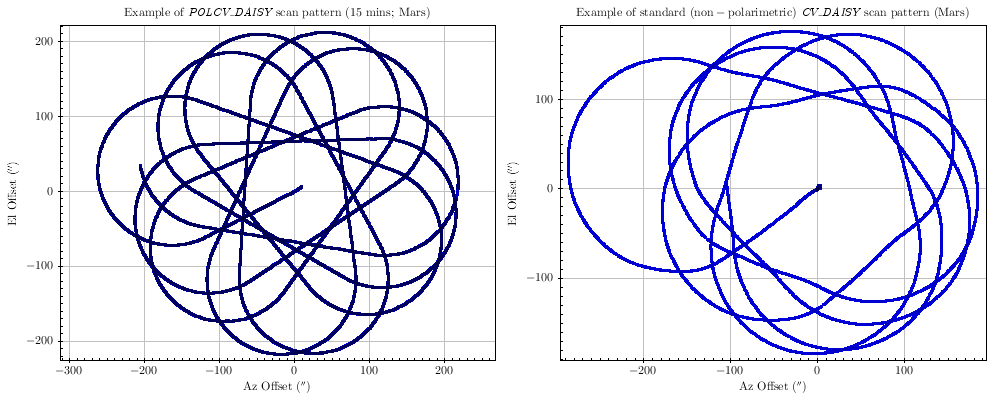
\includegraphics[width=0.9\linewidth]{scan_pattern_daisy_comparison.png}
\label{fig:scancompsrison}
\caption [Scan Pattern Comparison]{Left: Scan pattern from a typical
  SCUBA-2 CV\_Daisy observation. Right: Scan pattern from a POL-2
  Daisy. The standard POLCV\_DAISY scan parameters are given in Table
  \ref{tab:scanpar} }
\end{center}
\end{figure}


The telescope must scan slowly enough to obtain sufficient data at
each point on the sky to allow good $Q$ and $U$ values to be
determined. The current commissioned scan pattern has a size of
200\si{\arcsecond} and a scan speed of 8\si{\arcsecond}/s. The data
reduction splits the data stream into short segments and determines a
pair of $Q$ and $U$ values from each segment.

The length of each such data segment is the time it takes the
telescope to traverse a pixel in the generated map. With the current
scanning parameters this is 0.5 and 0.25 seconds for 850 and
\SI{450}{\micro\metre}, respectively. The modulation generated by any
polarisation is 8 Hz at the current HWP rotation speed (2 Hz).

The standard POLCV\_DAISY scan parameters are given in
Table~\ref{tab:scanpar} and shown in Figure~\ref{fig:scandetail}.

\begin{table}[h!]
\begin{center}
\begin{tabular}{r|l}
\hline
Parameter & Value\\
\hline
Half-wave plate rotation frequency& \SI{2}{Hz}\\
 Antenna scanning speed & 8\si{\arcsecond}/s\\
 R$_{0}$ (map pattern radius)\textdagger
& 133\si{\arcsecond}\\
 R$_{t}$ (turn radius) & 99\si{\arcsecond}\\
 R$_{a}$ (nominal avoidance radius) & 77\si{\arcsecond}\\
\hline
\end{tabular}
\caption{The scan parameters used in the POLCV\_DAISY
  mode. \textdagger This radius is \emph{not} the size of the
  resulting map. }
\label{tab:scanpar}
\end{center}
\end{table}


\begin{figure}[t!]
\begin{center}
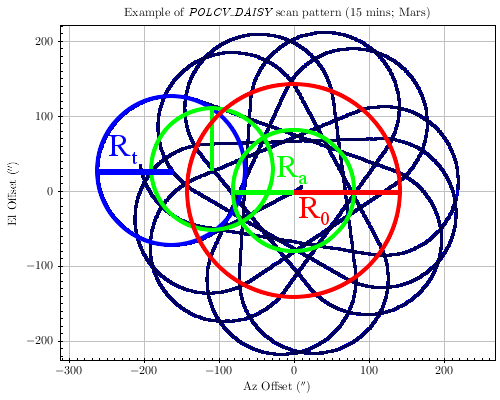
\includegraphics[width=0.6\linewidth]{POLCV_DAISY_schematic_detailed.png}
\caption [Detail of POL-2 Scan Pattern]{Detail of
  POLCV\_DAISY. $R_{0}$ is the map pattern radius, $R_{t}$ the turn
  radius, and $R_{a}$ is the nominal avoidance radius. For more
  details see Table~\ref{tab:scanpar}.}
\label{fig:scandetail}
\end{center}
\end{figure}


\section{The raw data}
\label{sec:rawdata}
SCUBA-2 is the detector for POL-2, and as such, the raw data format of
POL-2 data is the same as a typical SCUBA-2 observation. The sequence
for both observations is:

\begin{enumerate}\itemsep-0.2em
\item Dark noise
\item Flat-field
\item Science scans
\item Flat-field
\end{enumerate}


The \param{SEQ$\_$TYPE} keyword in the FITS header may be used to
identify the nature of each scan.  When you access raw data from the
CADC archive
\htmladdnormallink{http://www3.cadc-ccda.hia-iha.nrc-cnrc.gc.ca/jcmt/}\
you will get all of the files listed above.


Critically the \param{INBEAM} keyword in the FITS header may be used
to identify if POL-2 is in the beam, and hence differentiate between
SCUBA-2 and POL-2 observations.


\begin{tip}
  Use the \Kappa\ command fitslist to see all FITS headers in a
  particular NDF. To obtain a specific header simply use the command
  fitsval:
  \begin{terminalv}
% fitsval s8a20160112_00056_0001.sdf INBEAM
pol
\end{terminalv}
The FITS header information may also be viewed via the \gaia\ View /
FITS header drop-down menu option.
\end{tip}

Shown below is an incomplete list of the raw files for a single
sub-array (in this case s8a) for a short POL-2 observation. The first
and last scans are the flat-field observations,which occur after the
shutter opens to the sky at the start of the observation and closes at
the end (note the identical file size); all of the scans in between
are science scans.


\begin{terminalv}
% ls -lh /jcmtdata/raw/scuba2/s8a/20160112/00056
\end{terminalv}

\begin{terminalv}
-rw-r--r-- 1 jcmtarch jcmt 5.6M Jan 12  2016 s8a20160112_00056_0001.sdf
-rw-r--r-- 1 jcmtarch jcmt 7.9M Jan 12  2016 s8a20160112_00056_0002.sdf
-rw-r--r-- 1 jcmtarch jcmt  25M Jan 12  2016 s8a20160112_00056_0003.sdf
-rw-r--r-- 1 jcmtarch jcmt  25M Jan 12  2016 s8a20160112_00056_0004.sdf
-rw-r--r-- 1 jcmtarch jcmt  25M Jan 12  2016 s8a20160112_00056_0005.sdf
...
-rw-r--r-- 1 jcmtarch jcmt  25M Jan 12  2016 s8a20160112_00056_0025.sdf
-rw-r--r-- 1 jcmtarch jcmt  25M Jan 12  2016 s8a20160112_00056_0026.sdf
-rw-r--r-- 1 jcmtarch jcmt  25M Jan 12  2016 s8a20160112_00056_0027.sdf
-rw-r--r-- 1 jcmtarch jcmt  22M Jan 12  2016 s8a20160112_00056_0028.sdf
-rw-r--r-- 1 jcmtarch jcmt 7.9M Jan 12  2016 s8a20160112_00056_0029.sdf
\end{terminalv}

The SCUBA-2 data acquisition (DA) system writes out a data file every
30 seconds; each of which contains 22\,MB of data. The only exception
is the final science scan which will usually be smaller (7.9\,MB in
the example above), typically requiring less than 30 seconds of data
to complete the observation.

\textbf{Note:} All of these files are written out eight times, once
for each of the eight sub-arrays. It should also be noted that the
POL-2 instrument has not been released from commissioning at 450
$\mu$m.

The main data array in each NDF is a cube, with the first two
dimensions corresponding to bolometer columns and rows within a
sub-array, and the third dimension corresponding to time slice index
(sampled at roughly 200\,Hz).

A standardised file naming scheme is used in which each file name
starts with the sub-array name, followed by the UT date of the
observation in the format \texttt{yyyymmdd}, followed by a five-digit
observation number, followed by the sub-scan number. The name ends
with the standard suffix \texttt{.sdf} used by all Starlink NDF data
files. For instance, the files listed above hold data from the s8a
sub-array for observation 34 taken on 12\textsuperscript{th} January
2016.




\subsubsection*{Units/Calibration}

Raw POL-2 data come in uncalibrated units. The first calibration step
is to scale the raw data to units of pico Watts (pW) by applying the
flat-field solution. This step is performed internally by the SMURF
command calcqu - used to calculate I, Q and U time-streams from the
raw data - but can be done manually when examining the raw data.

If the purpose of a given POL-2 observation is to determine the
percentage polarisations or vector angles within a source/region of
interest then the data may remain in pW. On the other hand, if the
purpose is to establish the absolute polarised intensities then a
value for the Flux Conversion Factor (FCF) is required.

The resulting map may have the FCF applied to convert it into units of
Janskys. As is recommended with SCUBA-2 observing, it is advisable to
check that the FCF value applied to the data is sensible (and must be
done manually). For more details see
\cref{Chapter}{sec:pol2map-fcf}{POL-2 FCFs}.





